\section{Multilayer perceptron}


Dans cet exercice, nous devons implémenter un réseau de neurones. Pour faire cela, on doit indiquer le nombre d'entrées des features, le nombre de neurones présents dans la couche cachée et le nombre des sorties. Ensuite, il a fallu mettre en place le backpropagatoin trainer \texttt{BackPropTraing} qui s'occupe d'entraîner notre réseau de neurones avec le dataset de training et deux paramètres : le \texttt{momentum} et le \texttt{learning rate}. Pour commencer l'entraînement du réseau de neurones, on appelle ensuite \texttt{trainer.train()} qui exécute une \texttt{epoch} d'entrainement sur le réseau de neurones. Voici donc le code de cet exercice :

\lstinputlisting{code/FNN.py}
\newpage


Avec l'entraînement par défaut on comme résultat une \texttt{précision de 0.55}, un \texttt{recall de 0.67} et un \texttt{f-score de 0.60}. La matrice de confusion de la figure \ref{mat001} nous montre aussi que les classes ne sont pas bien reconnues par le classificateur.

\begin{figure}[h]
  \centering
    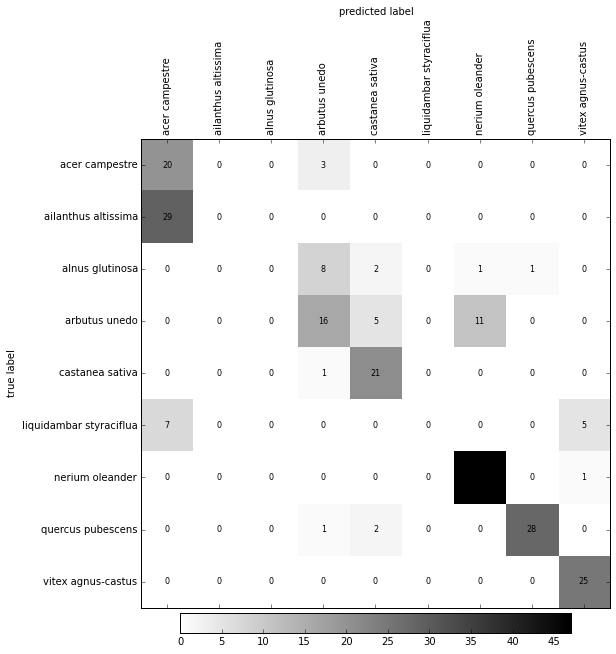
\includegraphics[width=0.6\linewidth]{img/mconf_001.png}
  \caption{Matrice de confusion avec learning rate 0.001 et 50 itérations}
  \label{mat001}
\end{figure}
\newpage


On a donc dû tuner ces paramètres pour améliorer les résultats. On a commencé par modifier le training rate a \texttt{trainintrate=0.2} pour chercher à améliorer plus rapidement l'erreur générée par l'entraînement et arriver a de meilleurs résultats. 


Par contre, comme on peut voir sur le graphique de la figure \ref{graph1}, l'erreur d'entraînement est assez instable, cela n'est pas optimal pour trouver une bonne convergence. 
\begin{figure}[h]
  \centering
    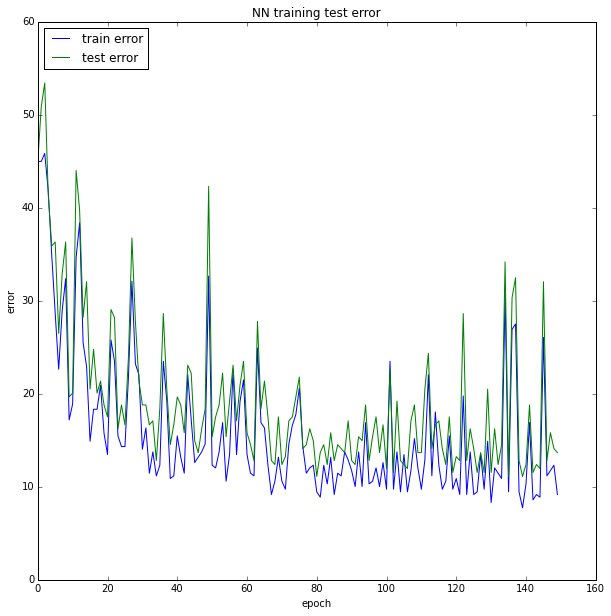
\includegraphics[width=0.6\linewidth]{img/graph3.png}
  \caption{Erreur d'entrainement et de test}
  \label{graph1}
\end{figure}
\newpage


Nous avons donc essayé plusieurs paramètres et avons trouvé certains qui paraîssent les meilleurs. Au final on a exécuté \texttt{150 itérations} avec un \texttt{momentum=0.1} et un \texttt{learningrate=0.03}. On a eu comme résultat une \texttt{precision de 0.82}, un \texttt{recall de 0.86} et un  \texttt{f-score de 0.84} que sont assez similaire aux résultats du KNN. Le graphique représenté par la figure \ref{graph003} nous montre que l'entraînement est plus stable qu' avant et qu' on arrive à la convergence. On pourrait en effet même diminuer le nombre d'itérations.

\begin{figure}[h]
  \centering
    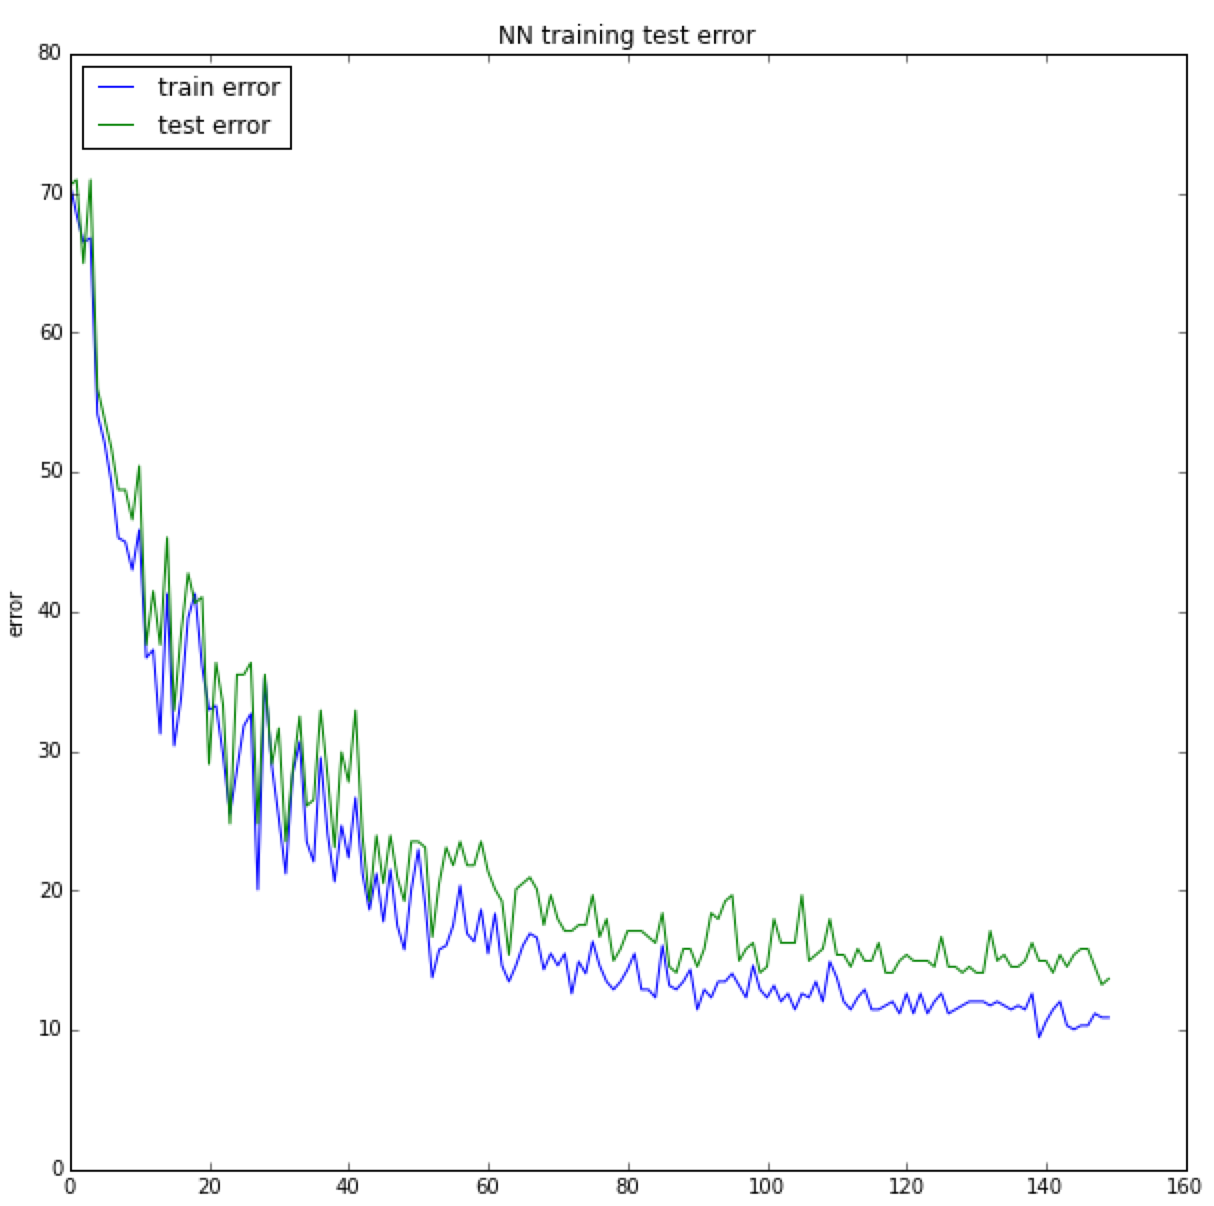
\includegraphics[width=0.6\linewidth]{img/graph003.png}
  \caption{Erreur d'entraînement et de test avec \texttt{training\_rate=0.003}}
  \label{graph003}
\end{figure}
\newpage

Au final la matrice de la figure \ref{mconf003} nous montre que les classes sont beaucoup mieux classées qu'avant et que, mis à part la classe \texttt{liquidambar styraciflue}, elles sont suffisamment bien reconnues par le classificateur.

\begin{figure}[h]
  \centering
    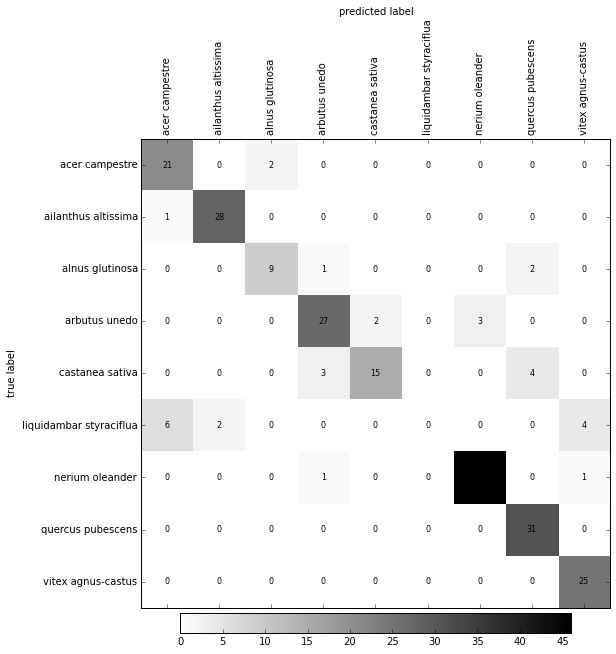
\includegraphics[width=0.6\linewidth]{img/mconf_003.png}
  \caption{Matrice de confusion finale}
  \label{mconf003}
\end{figure}



